\begin{figure}[H]
    \centering
    \begin{subfigure}{0.25\textwidth}
        \centering
        \includegraphics[width=0.9\textwidth]{rotacoes/64_alp_viz.png}
        \caption{~\texttt{vizinho}.}
    \end{subfigure}%
    \hspace{8pt}%
    \begin{subfigure}{0.25\textwidth}
        \centering
        \includegraphics[width=0.9\textwidth]{rotacoes/64_alp_bil.png}
        \caption{~\texttt{bilinear}.}
    \end{subfigure}
    \\[8pt]
    \begin{subfigure}{0.25\textwidth}
        \centering
        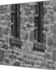
\includegraphics[width=0.9\textwidth]{rotacoes/64_alp_bic.png}
        \caption{~\texttt{bicubica}.}
    \end{subfigure}%
    \hspace{8pt}%
    \begin{subfigure}{0.25\textwidth}
        \centering
        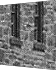
\includegraphics[width=0.9\textwidth]{rotacoes/64_alp_lag.png}
        \caption{~\texttt{lagrange}.}
    \end{subfigure}

    \caption{Rotação de -30\textdegree{} no plano da imagem aplicada em \texttt{house16.png} ($64 \times 64$).}
    \label{fig:rot:house64}
\end{figure}